\chapter{Requisitos do Sistema}

\section{Análise e Levantamento dos Requisitos}
A aplicação a desenvolver deverá suportar o registo das despesas e a gestão do seu pagamento por parte de moradores registados.

\subsection{Criação do grupo com os elementos da casa/apartamento}

\begin{itemize}
	

\item{Cada morador deve efetuar um registo fornecendo o seu nome, e-mail, número de telemóvel e data de nascimento.}

\item{O morador assim como o utilizador necessitam de efetuar login na aplicação}

\item{O utilizador que convidar os restantes será considerado adminstrador do sistema.} 

\end{itemize}

\subsection{Gestão das contas}

\begin{itemize}
	
\item{Após o registo será associada uma conta corrente a cada utilizador.}

\item{Cada conta corrente permitirá a gestão do saldo corrente (estão incluidas dívidas) de cada morador.}

\item{O morador deverá efetuar um pagamento.}
 
\item{Cada pagamento será creditado na conta corrente do morador.}
 
 \item{O pagamento pode ser igual ou superior à quantia necessária para pagar as despesas em causa.}
 
 
\item{Existirá um saldo global da casa, este que é o somatório de todas as contas correntes dos moradores}
 
 \item{O saldo global é administrado por um Adminstrador}
 
\item{Existem dois tipos de despesas distintos: a despesa recorrente referente a despesas mensais como a água, luz, renda, etc; a despesa extra referente a por exemplo arranjos de material na casa}
 
\item{Cada morador deverá pagar uma fração relativa à despesa}
 
\item{Cada despesa a pagar tem a si associado um tipo (i.e. água, luz, cadeiras, etc)}

\end{itemize}


\section{Base de dados }
A aplicação necessitará de uma implementação de uma base de dados para gerir os elementos que pertencem ao grupo assim como as despesas efetuadas pelos moradores. 

\chapter{Arquitetura da Aplicação}

\section{Modelo de Dominio }
Todo e qualquer projeto possui um domínio específico. O modelo de domínio deve capturar os seguintes pontos: as entidades, os relacionamentos entre as entidades e o vocabulário de domínio do problema. Para além disso também deve ser uma visão estática do problema onde é possível representar as regras de negócio invariantes no tempo. Ou seja, o modelo de domínio é a base para a análise de requisitos.

No que diz respeito à aplicação, como é dito na introdução, queremos desenvolver uma aplicação capaz de suportar o registo das despesas e a gestão do seu pagamento por parte dos moradores registados.


\begin{figure}[htb!]
	\includegraphics[scale=0.4]{imagens/mD/"ModeloDominio"}  
	\caption{Modelo Dominio}  
\end{figure}

O morador necessita de fornecer o nome, e-mail, número de telemovel e data de nascimento, para efetuar o login. 

Como se pode observar na figura o morador efetua pagamento relativo a despesa recorrente ou extra, assim como paga uma fração da despesa, essa fração é relativa a um tipo de despesa. 


O administrador administra o saldo global da casa/apartamento. 


\newpage

\section{Modelo de Use Case}
A segunda parte da análise de requisitos corresponde à definição dos use cases, com o objetivo de os aplicar nesta primeira fase deste trabalho prático. Nos use cases, queremos primeiramente, identificar os atores, que serão quem interagirá com o sistema.
Posterior à identificação dos atores, passamos então à identificação dos use cases, isto é, o que se pretende do sistema. No último ponto da visão orientada aos use cases, procedemos à identificação das classes de suporte à realização dos mesmo, que corresponde à especificação da funcionalidade a ser implementada.
Neste sentido, quando definimos um use case, para além de ser uma espécie de documentação, temos de ter em conta que se trata de uma unidade coerente de funcionalidade, um serviço. Define também um comportamento do sistema, sem revelar a estrutura interna, divulgando desta forma, a comunicação entre os atores e o sistema.
O conjunto de todos os use cases acaba por definir pela íntegra, toda a funcionalidade do sistema que decorre na sua essência, do diálogo entre o sistema e os atores, e a responsabilidade de resposta funcional do sistema.



\subsection{Diagrama de Use Case}


\begin{figure}[htb!]
	\centering
	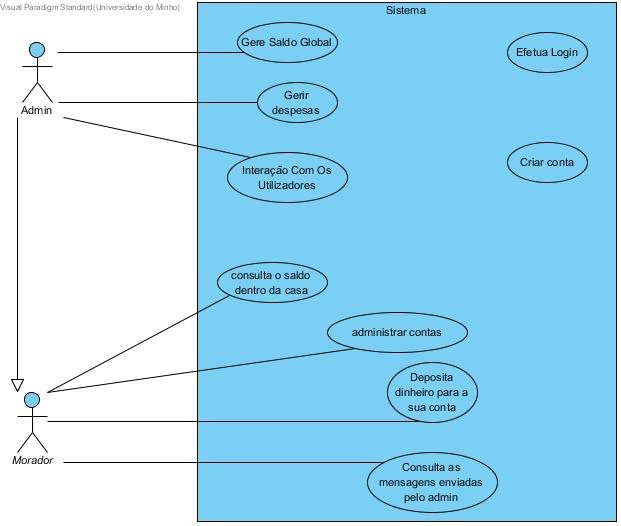
\includegraphics[scale=0.5]{UseCase}  
	\caption{Modelo Use Case}  
\end{figure}

\newpage
\subsubsection{Especificação: Gere Saldo Global }

\begin{figure}[htb!]
	\centering
	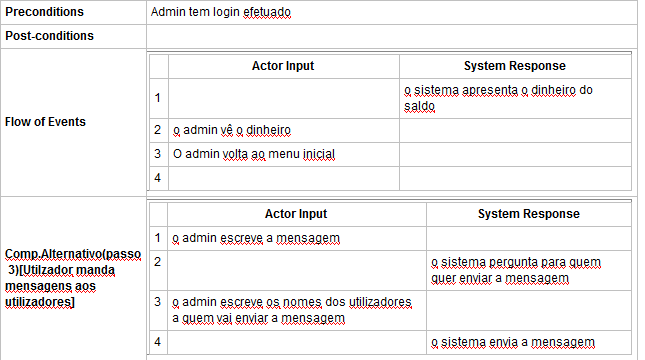
\includegraphics[scale=0.6]{imagens/Especificacoes/geresaldoglobal}  
	\caption{Especificação do Use Case: Gere Saldo Global  }  
\end{figure}


\subsubsection{Especificação: Efetua Login }

\begin{figure}[htb!]
	\centering
	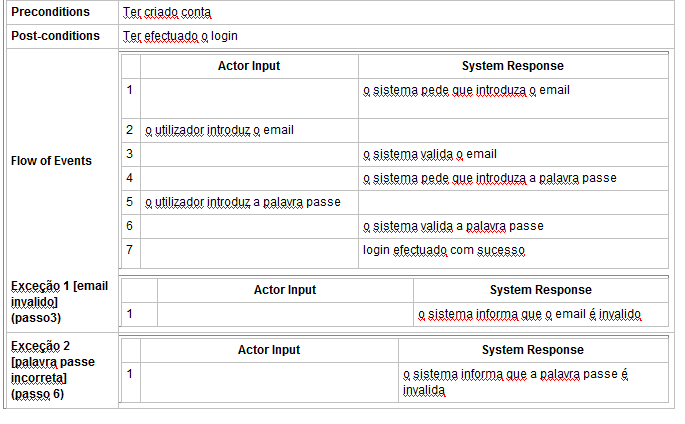
\includegraphics[scale=0.6]{imagens/Especificacoes/efetualogin}  
	\caption{Especificação do Use Case: Efetua Login  }  
\end{figure}

\newpage

\subsubsection{Especificação: Criar Conta }
\begin{figure}[htb!]
	\centering
	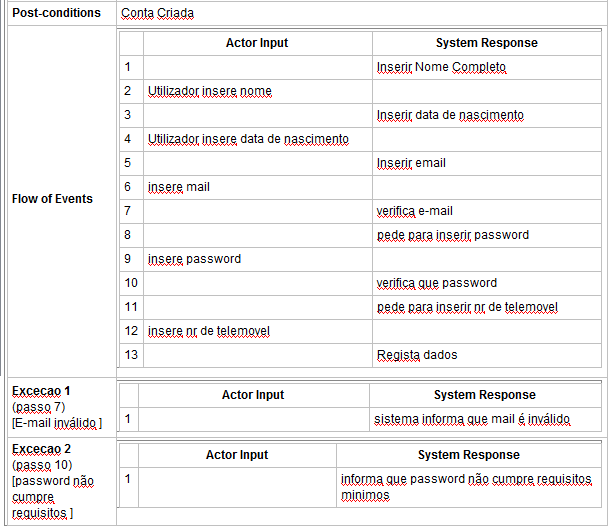
\includegraphics[scale=0.6]{imagens/Especificacoes/criarconta}  
	\caption{Especificação do Use Case: Criar Conta   }  
\end{figure}

\subsubsection{Especificação: Consulta Saldo dentro de casa }
\begin{figure}[htb!]
	\centering
	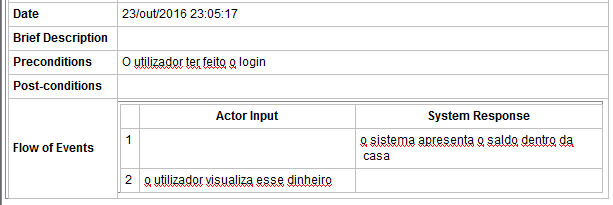
\includegraphics[scale=0.6]{imagens/Especificacoes/consultasaldodentrodecasa}  
	\caption{Especificação do Use Case: Consulta Saldo dentro de Casa   }  
\end{figure}

\newpage

\subsubsection{Especificação: Deposita Dinheiro para a sua Conta }
\begin{figure}[htb!]
	\centering
	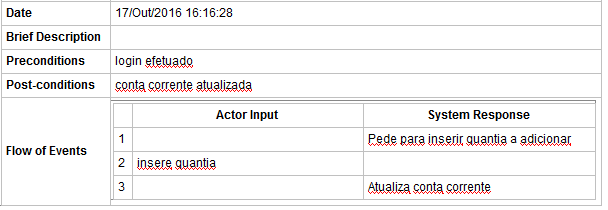
\includegraphics[scale=0.6]{imagens/Especificacoes/depositadinheiro}  
	\caption{Especificação do Use Case: Deposita Dinheiro para a sua conta  }  
\end{figure}

\subsubsection{Especificação: Consulta Mensagens enviadas pelo Administrador }
\begin{figure}[htb!]
	\centering
	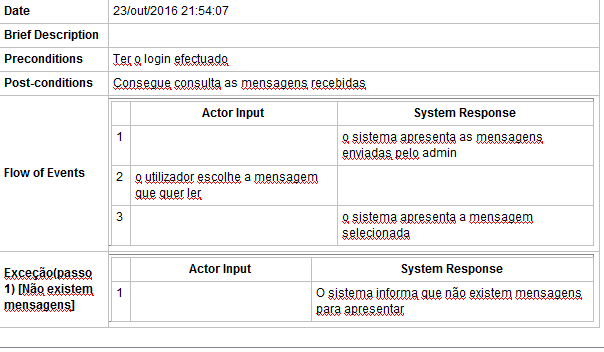
\includegraphics[scale=0.6]{imagens/Especificacoes/consultasmsadmin}  
	\caption{Especificação do Use Case: Consulta Mensagens enviadas pelo Administrador}  
\end{figure}

\newpage
\subsection{Subdiagrama Gerir Despesas}

\begin{figure}[htb!]
	\centering
	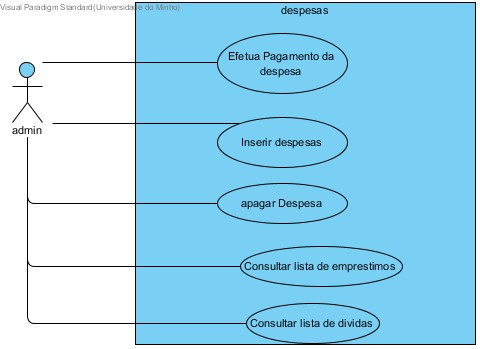
\includegraphics[scale=0.5]{imagens/UseCase/GerirDespesas}  
	\caption{Sub-Diagrama Gerir Despesas }  
\end{figure}

\subsubsection{Especificação: Efetua pagamento da despesa}

\begin{figure}[htb!]
	\centering
	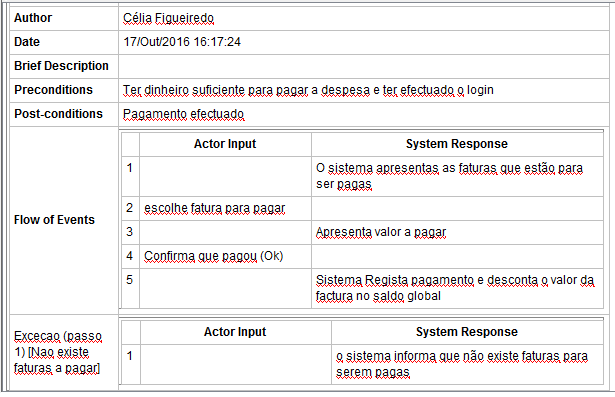
\includegraphics[scale=0.6]{imagens/Especificacoes/efetuapagdespesa}  
	\caption{Especificação do Use Case:Efetua Pagamento da despesa  }  
\end{figure}

\newpage

\subsubsection{Especificação: Inserir Despesa}
\begin{figure}[htb!]
	\centering
	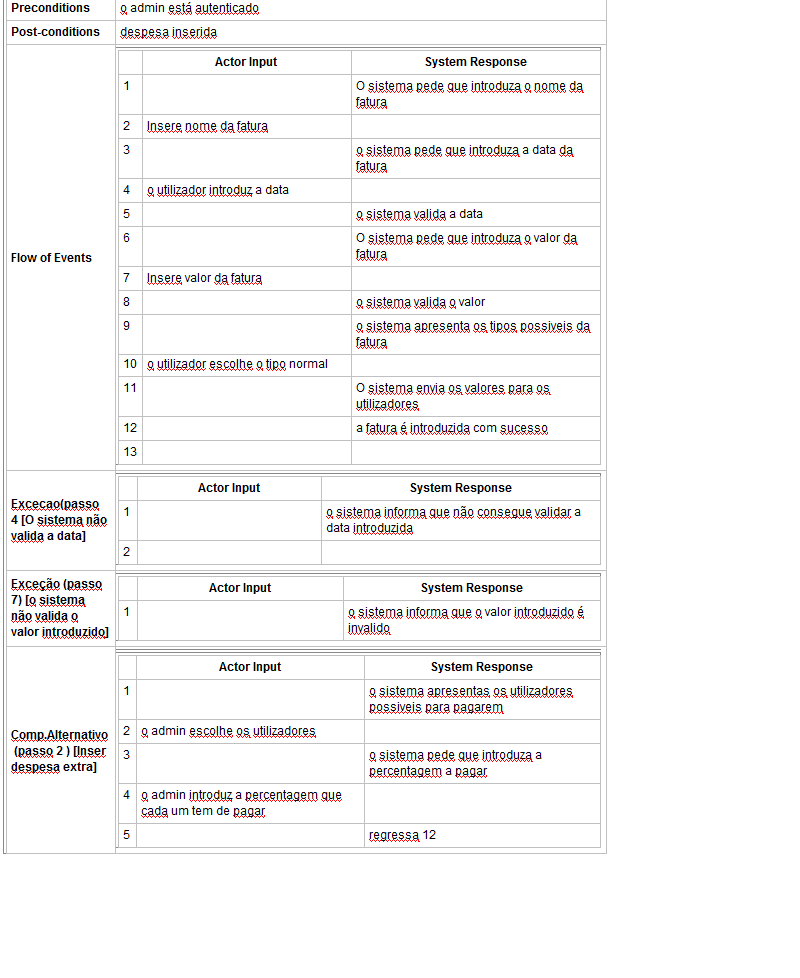
\includegraphics[scale=0.8]{imagens/Especificacoes/inserirdespesas}  
	\caption{Especificação do Use Case: Inserir Despesas}  
\end{figure}

\newpage

\subsubsection{Especificação: Apagar Despesa}

\begin{figure}[htb!]
	\centering
	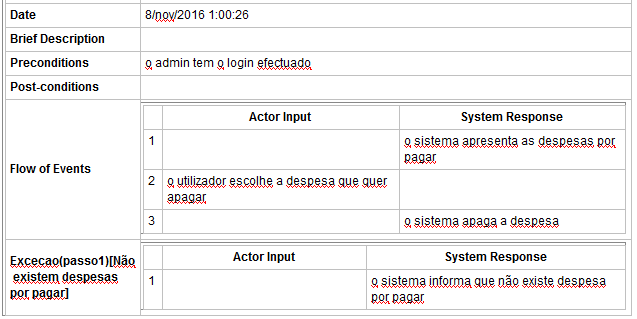
\includegraphics[scale=0.6]{imagens/Especificacoes/apagardespesa}  
	\caption{Especificação do Use Case: Apagar Despesa}  
\end{figure}


\subsection{Subdiagrama Administrar Contas}
\begin{figure}[htb!]
	\centering
	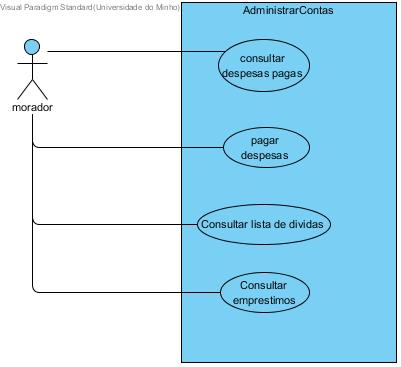
\includegraphics[scale=0.6]{imagens/UseCase/despesasMorador}  
	\caption{Subdiagrama: Administrar Contas }  
\end{figure}

\newpage

\subsubsection{Especificação: Consultar despesas pagas }

\begin{figure}[htb!]
	\centering
	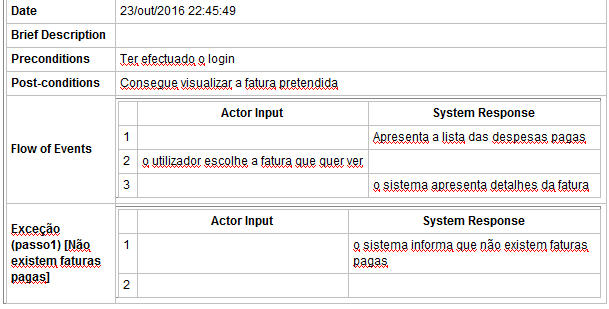
\includegraphics[scale=0.6]{imagens/Especificacoes/consultardespesaspagas}  
	\caption{Especificação do Use Case: Consultar Despesas Pagas}  
\end{figure}

\subsubsection{Especificação: Pagar Despesas }

\begin{figure}[htb!]
	\centering
	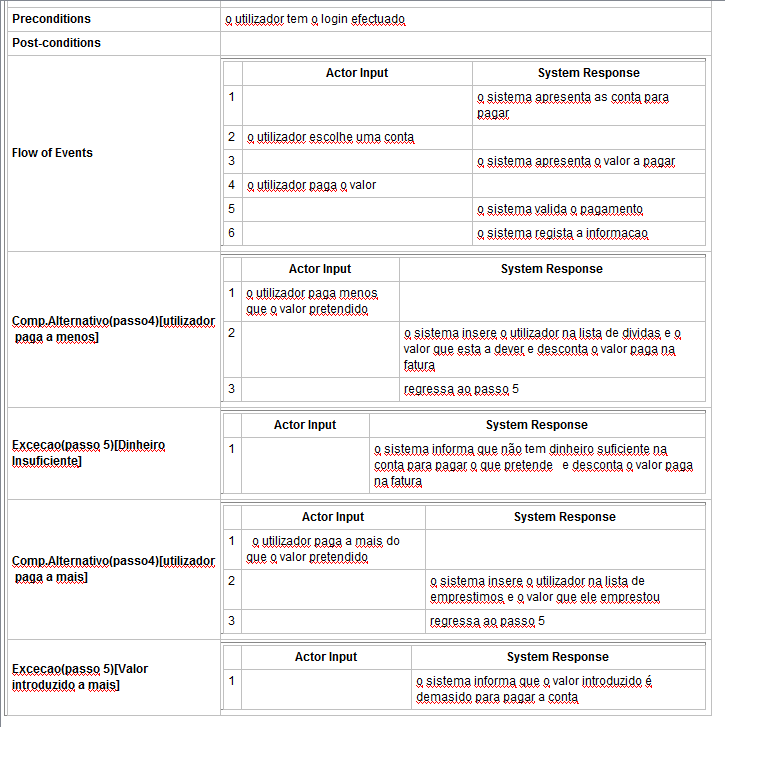
\includegraphics[scale=0.6]{imagens/Especificacoes/pagardespesas}  
	\caption{Especificação do Use Case: Pagar Despesas}  
\end{figure}

\newpage
\subsubsection{Especificação: Consultar Lista de Dívidas }

\begin{figure}[htb!]
	\centering
	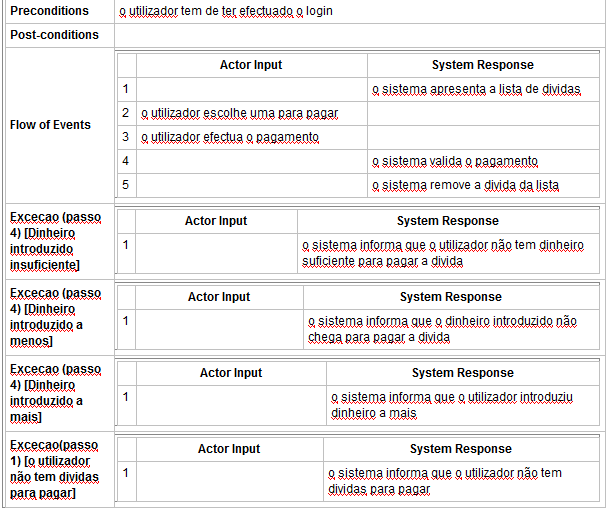
\includegraphics[scale=0.7]{imagens/Especificacoes/consultarlistadedividas}  
	\caption{Especificação do Use Case: Consultar lista de dividas}  
\end{figure}

\subsubsection{Especificação: Consultar Empréstimos }

\begin{figure}[htb!]
	\centering
	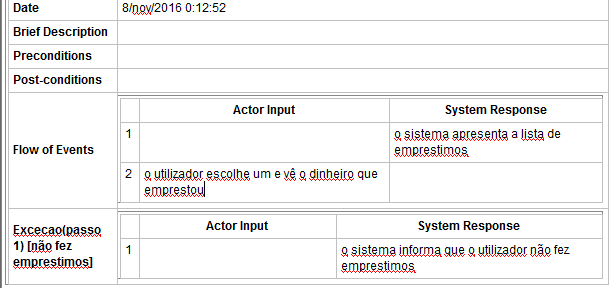
\includegraphics[scale=0.7]{imagens/Especificacoes/consultaremprestimos}  
	\caption{Especificação do Use Case: Consultar Empréstimos}  
\end{figure}

\newpage

\subsection{Subdiagrama Interação com os Utilizadores}
\begin{figure}[htb!]
	\centering
	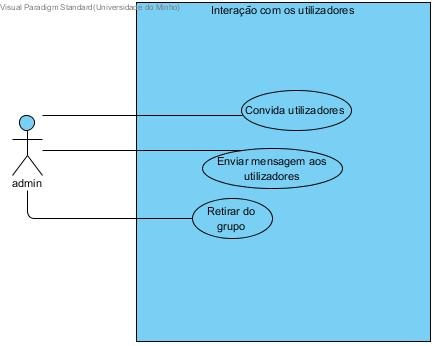
\includegraphics[scale=0.6]{imagens/UseCase/InteracaoComOsUtilizadores}  
	\caption{Subdiagrama: Interação com os utilizadores }  
\end{figure}

\subsubsection{Especificação: Convida Utilizadores }

\begin{figure}[htb!]
	\centering
	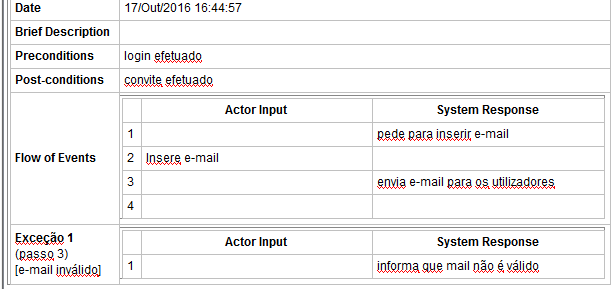
\includegraphics[scale=0.7]{imagens/Especificacoes/convidautilizadores}  
	\caption{Especificação do Use Case: Convida Utilizadores}  
\end{figure}

\newpage

\subsubsection{Especificação: Envia Mensagens aos Utilizadores }

\begin{figure}[htb!]
	\centering
	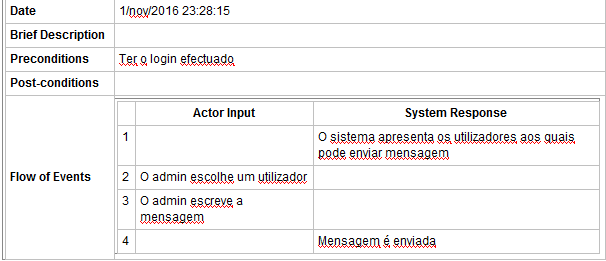
\includegraphics[scale=0.7]{imagens/Especificacoes/enviasmsutilizadores}  
	\caption{Especificação do Use Case: Envia Mensagens aos Utilizadores}  
\end{figure}



\subsubsection{Especificação: Retirar do grupo }

\begin{figure}[htb!]
	\centering
	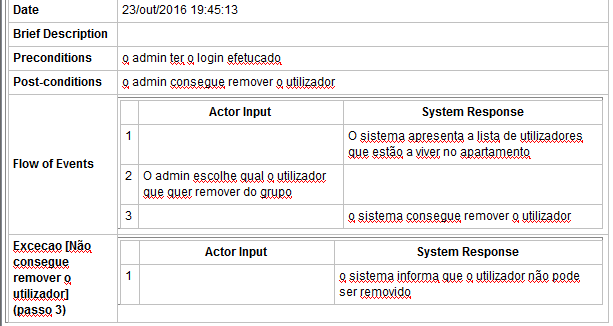
\includegraphics[scale=0.7]{imagens/Especificacoes/retirardogrupo}  
	\caption{Especificação do Use Case: Retirar do grupo}  
\end{figure}

\section{Máquinas de Estado}
\subsection{Efetuar Login}

\begin{figure}[htb!]
	\centering
	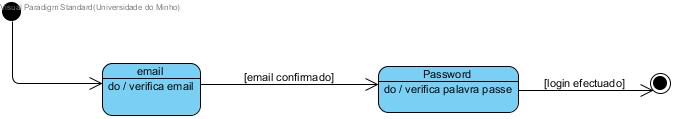
\includegraphics[scale=0.7]{imagens/maqEstados/Login}  
	\caption{Máquina de Estados: Efetuar Login}  
\end{figure}


\subsection{Criar Conta}
\begin{figure}[htb!]
	\centering
	\includegraphics[scale=0.55]{imagens/maqEstados/"Criar Conta"}  
	\caption{Máquina de Estados: Criar Conta}  
\end{figure}

\subsection{Convidar Utilizadores}
\begin{figure}[htb!]
	\centering
	\includegraphics[scale=0.45]{imagens/maqEstados/"Convidar Utilizadores"}  
	\caption{Máquina de Estados: Convidar Utilizadores}  
\end{figure}

\newpage

\subsection{Remover Utilizadores}
\begin{figure}[htb!]
	\centering
	\includegraphics[scale=0.45]{imagens/maqEstados/"Remover Utilizadores"}  
	\caption{Máquina de Estados: Remover Utilizadores}  
\end{figure}

\subsection{Inserir Fatura}
\begin{figure}[htb!]
	\centering
	\includegraphics[scale=0.45]{imagens/maqEstados/"InserFactura"}  
	\caption{Máquina de Estados: Inserir Fatura}  
\end{figure}

\subsection{Deposita Dinheiro}
\begin{figure}[htb!]
	\centering
	\includegraphics[scale=0.45]{imagens/maqEstados/"Deposita Dinheiro"}  
	\caption{Máquina de Estados: Deposita Dinheiro}  
\end{figure}

\newpage
\section{Mockups}
Apresentamos de seguida uma proposta de interface com o utilizador. Utilizámos o programa 'Pencil' para nos auxiliar na construção de uma possivel interface com o utilizador. 


Como já refirmos, para o utilizador efetuar o login necessita de se registar previamente, fornecendo alguns dados que o identifiquem. 
\begin{figure}[htb!]
	\centering
	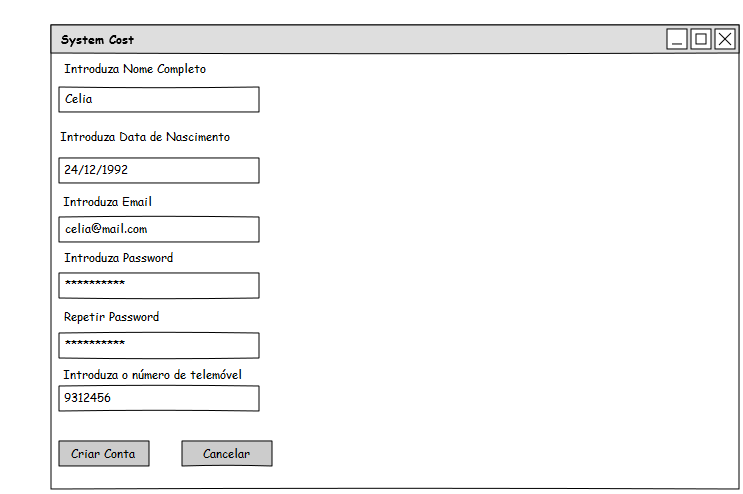
\includegraphics[scale=0.5]{imagens/mockups/CriarConta}  
	\caption{Criar nova Conta }  
\end{figure}

Esta será a janela para os moradores e administrador efetuarem login na aplicação. 
\begin{figure}[htb!]
	\centering
	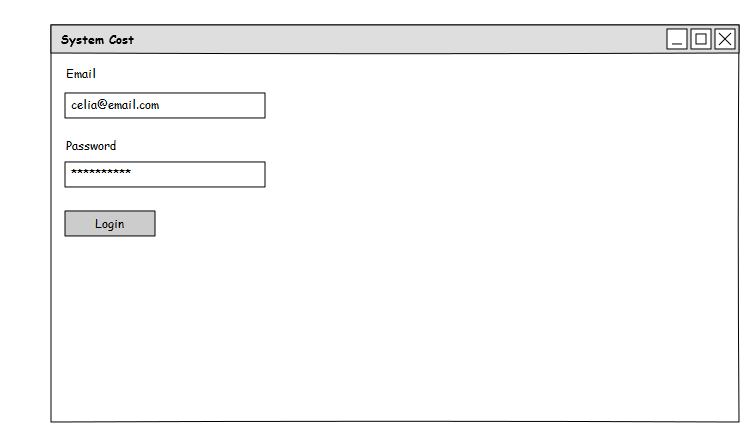
\includegraphics[scale=0.5]{imagens/mockups/MLogin}  
	\caption{Login}  
\end{figure}

\newpage
O Administrador efetua login, mas ainda não existem grupo criado. Pode escolher a opção "Convidar Pessoas", para iniciar a formação de um grupo. 
\begin{figure}[h!]
	\centering
	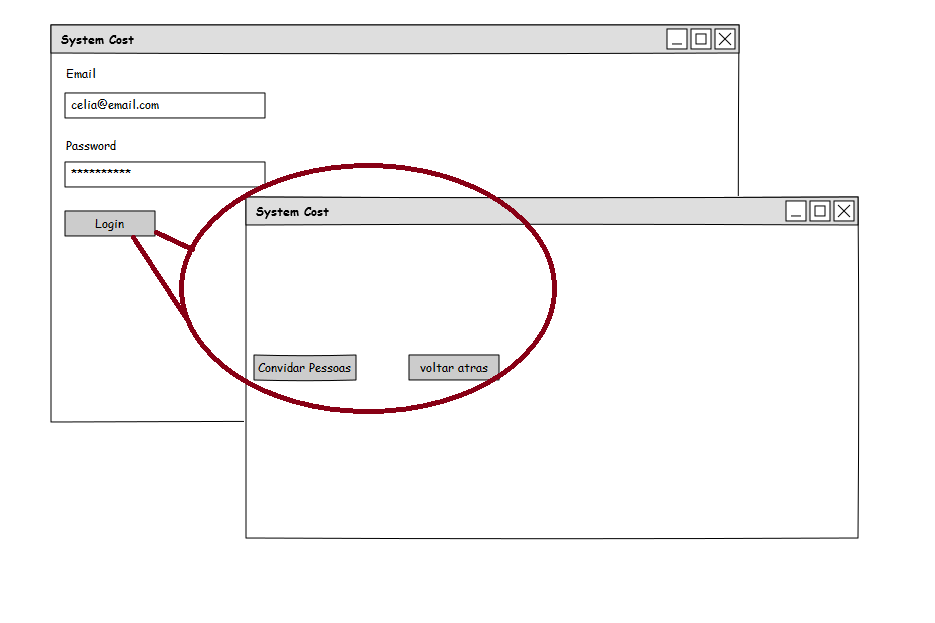
\includegraphics[scale=0.5]{imagens/mockups/loginsemgrupos}  
	\caption{Login quando não existem grupos criados }  
\end{figure}


Haverá sempre a possibilidade de ver/alterar os campos preenchidos inicialmente. 
Carregando no botão grupo abre uma janela onde se pode entrar para grupo constituido pelos elementos da casa/apartamento. Após clicar no botao "Entrar no grupo" é  apresentada uma lista com as pessoas já existentes e a possibilidade de convidar mais membros. 

\begin{figure}[htb!]
	\centering
	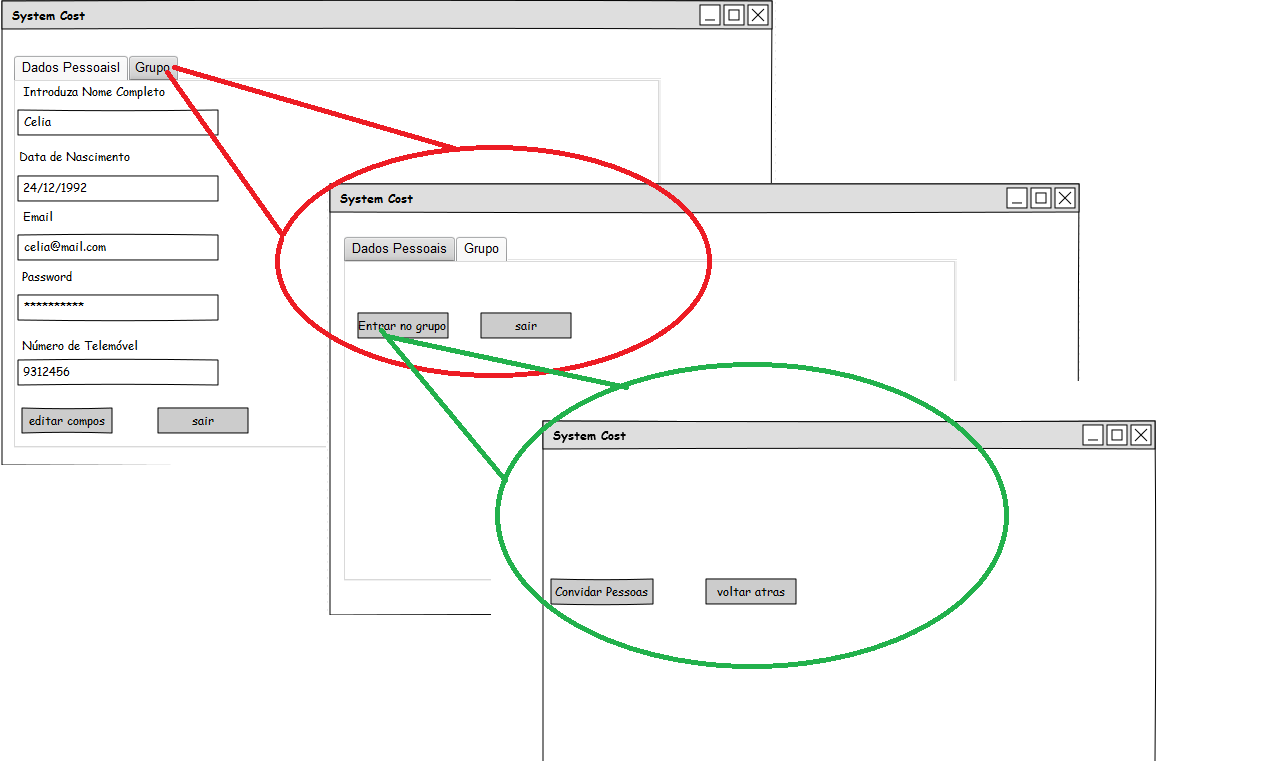
\includegraphics[scale=0.45]{imagens/mockups/consultardados}  
	\caption{Visualização/Alteração dos dados }  
\end{figure}


Após o utililizador efetuar o login é-lhe apresentada uma janela com as funcionalidades que a aplicação lhe oferece, como por exemplo pagar contas e acesso à lista de dividas, assim como o valor da conta corrente. 

\begin{figure}[htb!]
	\centering
	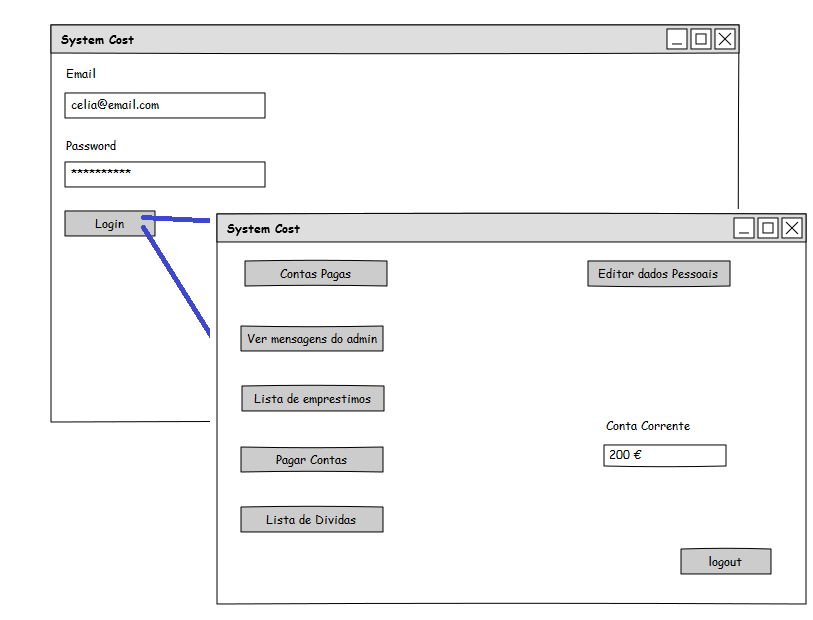
\includegraphics[scale=0.5]{imagens/mockups/logUtilizador}  
	\caption{Login /página inicial morador}  
\end{figure}

\begin{figure}[h!]
	\centering
	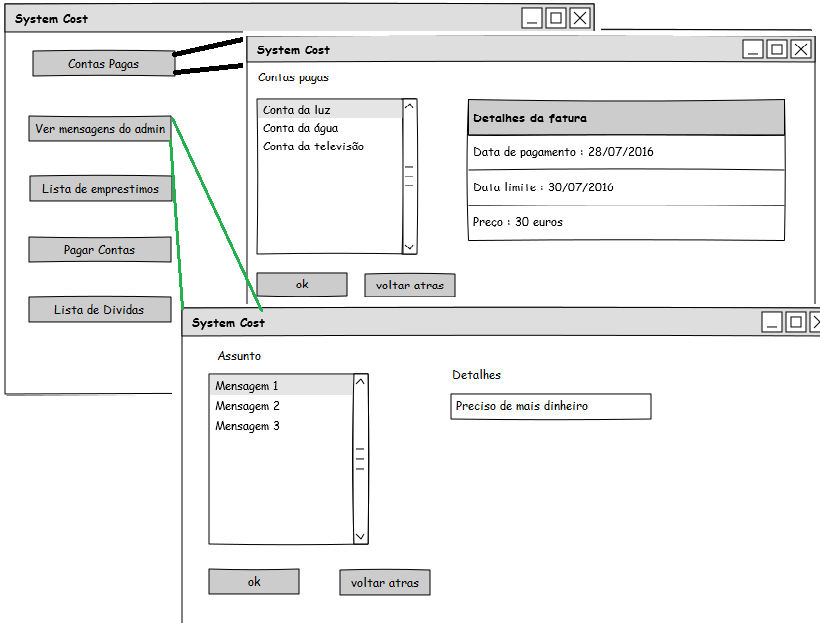
\includegraphics[scale=0.5]{imagens/mockups/tarefasutilizador}  
	\caption{Opções do utilizador }  
\end{figure}

\newpage
Após o administador efetuar o login é-lhe apresentada uma janela com as funcionalidades que a aplicação lhe oferece, como por exemplo pagar contas e adicionar/remover utilizador, enviar mensagem e verificar o saldo global

\begin{figure}[h!]
	\centering
	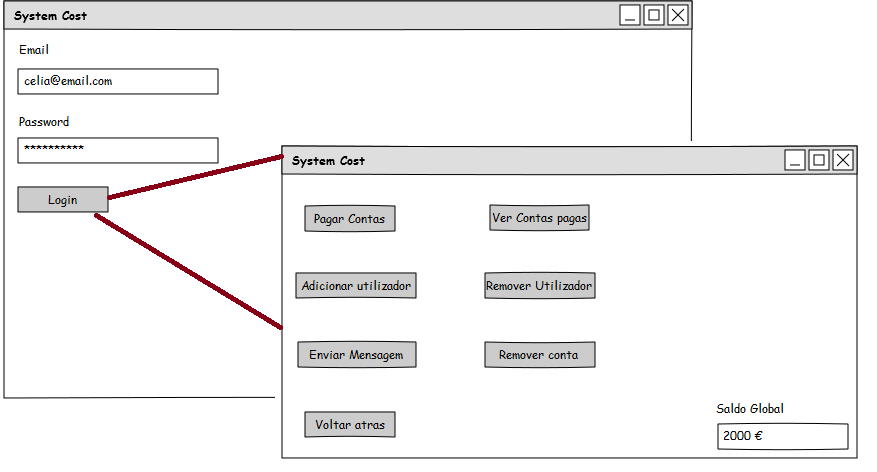
\includegraphics[scale=0.5]{imagens/mockups/loginadmin}  
	\caption{Login/Privilégios de administrador }  
\end{figure}


\begin{figure}[h!]
	\centering
	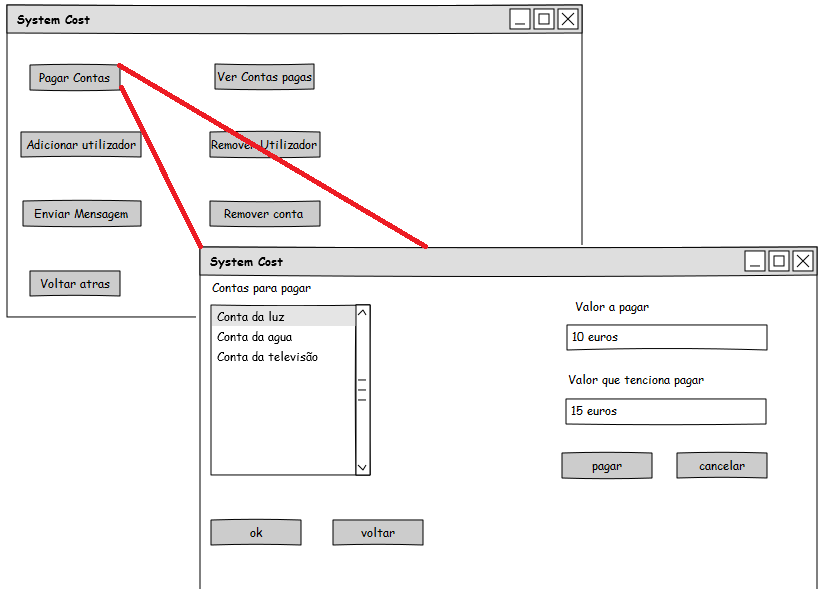
\includegraphics[scale=0.6]{imagens/mockups/AdminpagarContas}  
	\caption{Interface do administrador, janela pagar contas }  
\end{figure}










